\documentclass{article}
\usepackage[paperheight=39.333in,paperwidth=21.181in,margin=0in]{geometry}
\usepackage[sfdefault]{roboto}
\usepackage{graphicx}
\usepackage{tikz}
\usepackage[absolute,overlay]{textpos}
    \setlength{\TPHorizModule}{1in}
    \setlength{\TPVertModule}{1in}
\begin{document}
\begin{textblock}{13}(0.000,0.000)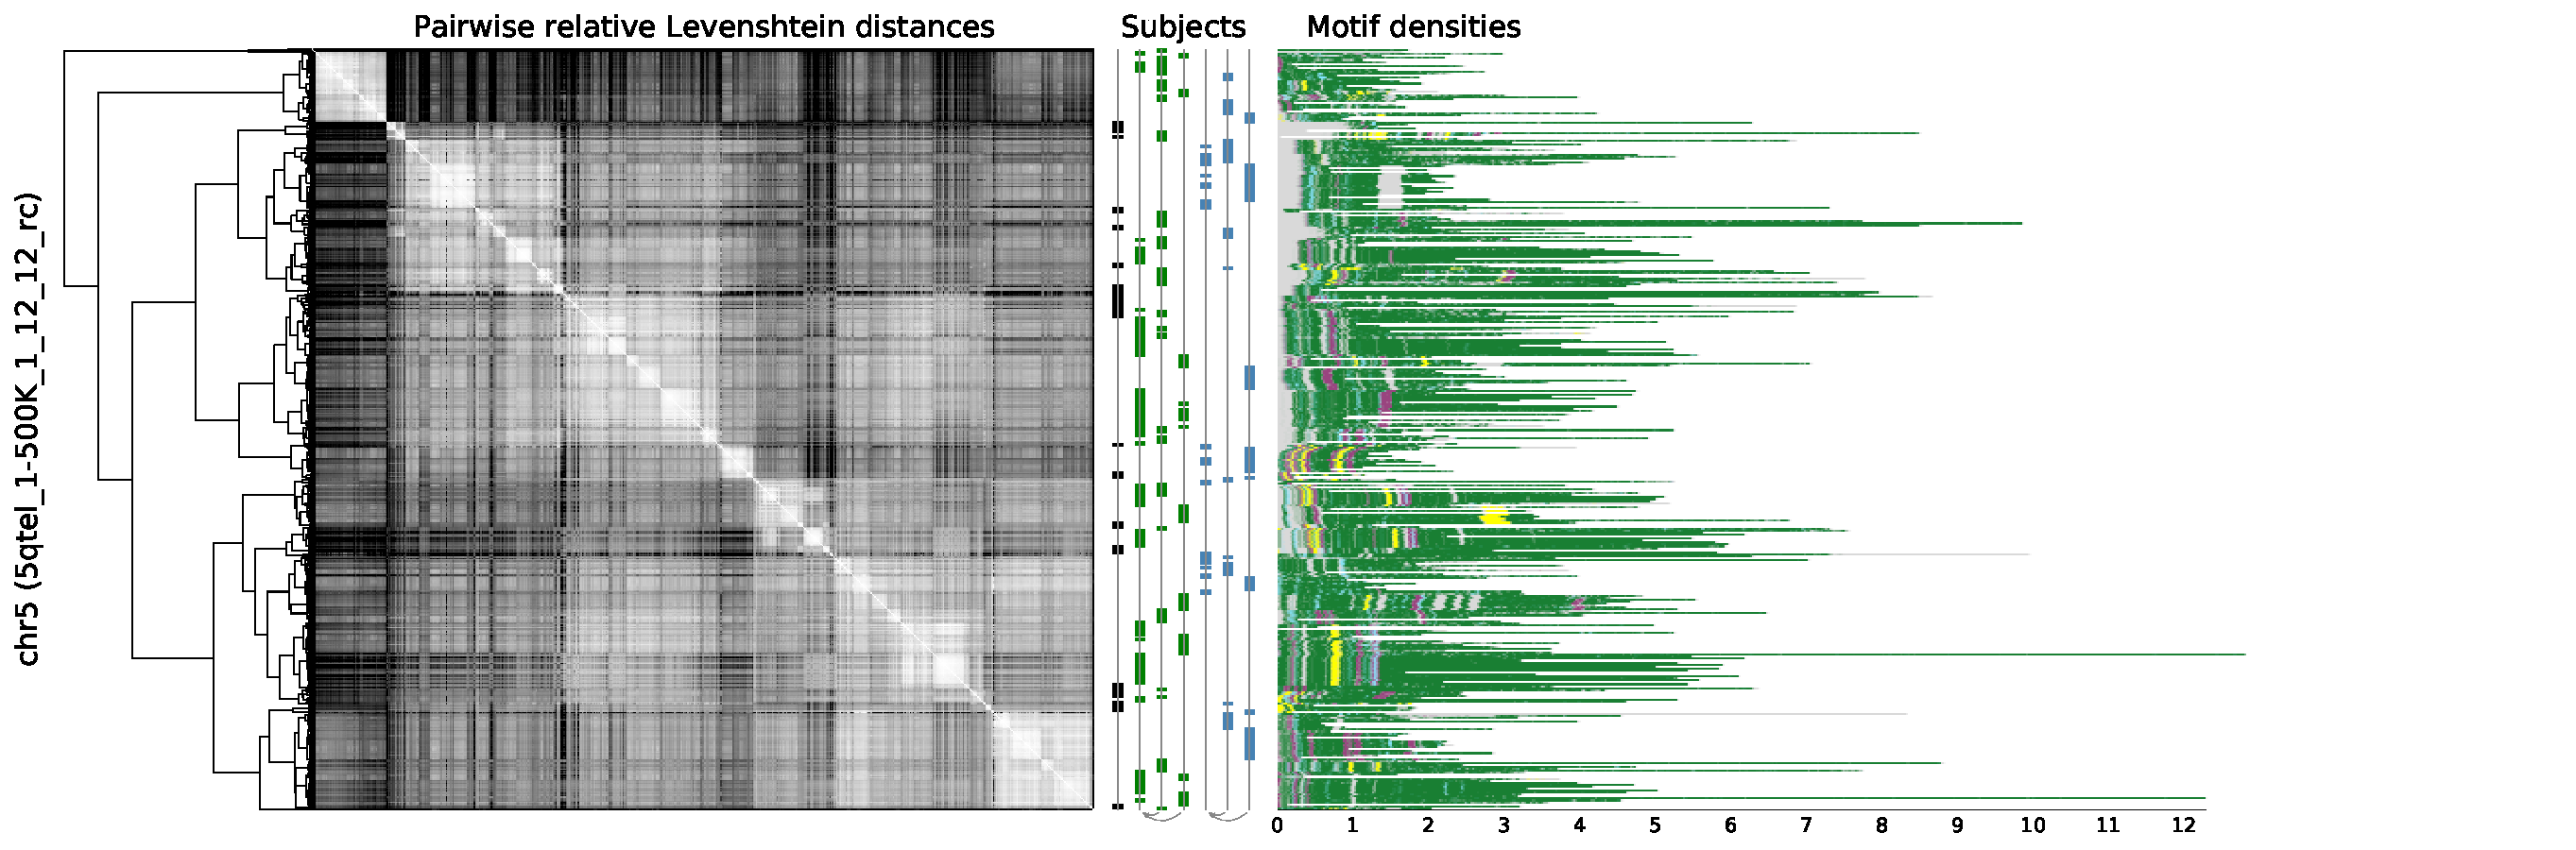
\includegraphics{latex/figures/haplotypes/5qtel_1-500K_1_12_12_rc.pdf}\end{textblock}
\begin{textblock}{13}(2.458,6.000)\includegraphics{latex/figures/haplotypes/6qtel_1-500K_1_12_12_rc.pdf}\end{textblock}
\begin{textblock}{13}(4.847,9.958)\includegraphics{latex/figures/haplotypes/chr7.pdf}\end{textblock}
\begin{textblock}{13}(4.528,12.181)\includegraphics{latex/figures/haplotypes/chr8.pdf}\end{textblock}
\begin{textblock}{13}(4.500,14.639)\includegraphics{latex/figures/haplotypes/chr11.pdf}\end{textblock}
\begin{textblock}{13}(4.861,17.111)\includegraphics{latex/figures/haplotypes/chr12.pdf}\end{textblock}
\begin{textblock}{13}(5.403,19.319)\includegraphics{latex/figures/haplotypes/14qtel_1-500K_1_12_12_rc.pdf}\end{textblock}
\begin{textblock}{13}(3.417,21.139)\includegraphics{latex/figures/haplotypes/chr15.pdf}\end{textblock}
\begin{textblock}{13}(5.778,24.417)\includegraphics{latex/figures/haplotypes/16qtel_1-500K_1_12_12_rc.pdf}\end{textblock}
\begin{textblock}{13}(5.569,25.069)\includegraphics{latex/figures/haplotypes/18qtel_1-500K_1_12_12_rc.pdf}\end{textblock}
\begin{textblock}{13}(6.208,26.819)\includegraphics{latex/figures/haplotypes/chr19.pdf}\end{textblock}
\begin{textblock}{13}(2.000,28.042)\includegraphics{latex/figures/haplotypes/chr21.pdf}\end{textblock}
\begin{textblock}{13}(2.889,32.347)\includegraphics{latex/figures/haplotypes/chr22.pdf}\end{textblock}
\begin{textblock}{13}(3.861,36.000)\includegraphics{latex/figures/haplotypes/chrX.pdf}\end{textblock}
\begin{textblock}{13}(16.456,0)
\includegraphics[width=4.500in,keepaspectratio]{latex/figures/haplotypes/haplotypes-legend.pdf}
\end{textblock}
\end{document}
